%%%% Proceedings format for most of ACM conferences (with the exceptions listed below) and all ICPS volumes.
\documentclass[sigconf]{acmart}
%%%% As of March 2017, [siggraph] is no longer used. Please use sigconf (above) for SIGGRAPH conferences.

%%%% Proceedings format for SIGPLAN conferences 
% \documentclass[sigplan, anonymous, review]{acmart}

%%%% Proceedings format for SIGCHI conferences
% \documentclass[sigchi, review]{acmart}

%%%% To use the SIGCHI extended abstract template, please visit
% https://www.overleaf.com/read/zzzfqvkmrfzn

\usepackage{booktabs} % For formal tables
\usepackage[utf8]{inputenc}
\usepackage{balance}


% Copyright
\setcopyright{none}
%\setcopyright{acmcopyright}
%\setcopyright{acmlicensed}
%setcopyright{rightsretained}
%\setcopyright{usgov}
%\setcopyright{usgovmixed}
%\setcopyright{cagov}
%\setcopyright{cagovmixed}

% DOI
\acmDOI{xx.xxx/xxx_x}

% ISBN
\acmISBN{xxx-xxxx-xx-xxx/xx/xx}

%Conference
\acmConference[Universidad Eafit]{}{May 2017}{Antioquia, Colombia}

\acmYear{2017}
\acmPrice{0.00}

\begin{document}
\title{A method for reconstructing DNA using a list of smaller DNA sequences}
%\titlenote{Produces the permission block, and
%  copyright information}
%\subtitle{Extended Abstract}
%\subtitlenote{The full version of the author's guide is available as
%  \texttt{acmart.pdf} document}

\author{Sebastián Patiño Barrientos}
\affiliation{%
  \institution{Universidad Eafit}
  \country{Colombia} 
}
\email{spatino6@eafit.edu.co}

\author{Luis Miguel Arroyave Quiñones}
\affiliation{%
  \institution{Universidad Eafit}
  \country{Colombia} 
}
\email{larroy13@eafit.edu.co}

\author{Juan José Jaramillo Castaño}
\affiliation{%
  \institution{Universidad Eafit}
  \country{Colombia} 
}
\email{jujara40@eafit.edu.co}

\author{Mauricio Toro}
\affiliation{%
  \institution{Universidad Eafit}
  \country{Colombia} 
}
\email{mtorobe@eafit.edu.co}

\renewcommand{\shortauthors}{S. Patiño, Luis M. Arroyave, JJ. Jaramillo, M. Toro}


\begin{abstract}
The idea of making optimal and each time better solutions to the problems that affect the humanity has been at the top goals of our generation, especially in the fields of computations and development of algorithms, as a record of that, we have the Needleman–Wunsch algorithm one of the first DP (dynamic programming) algorithms used in bioinformatics and computational genomics. Having said that, we can present the goal of this paper which is present an algorithmic solution to the problem of DNA sequence reconstruction using a collection of fragments and determine to which specie is it from.
\end{abstract}

%% Used in some conference proceedings e.g. sigplan and sigchi
% \begin{teaserfigure}
%   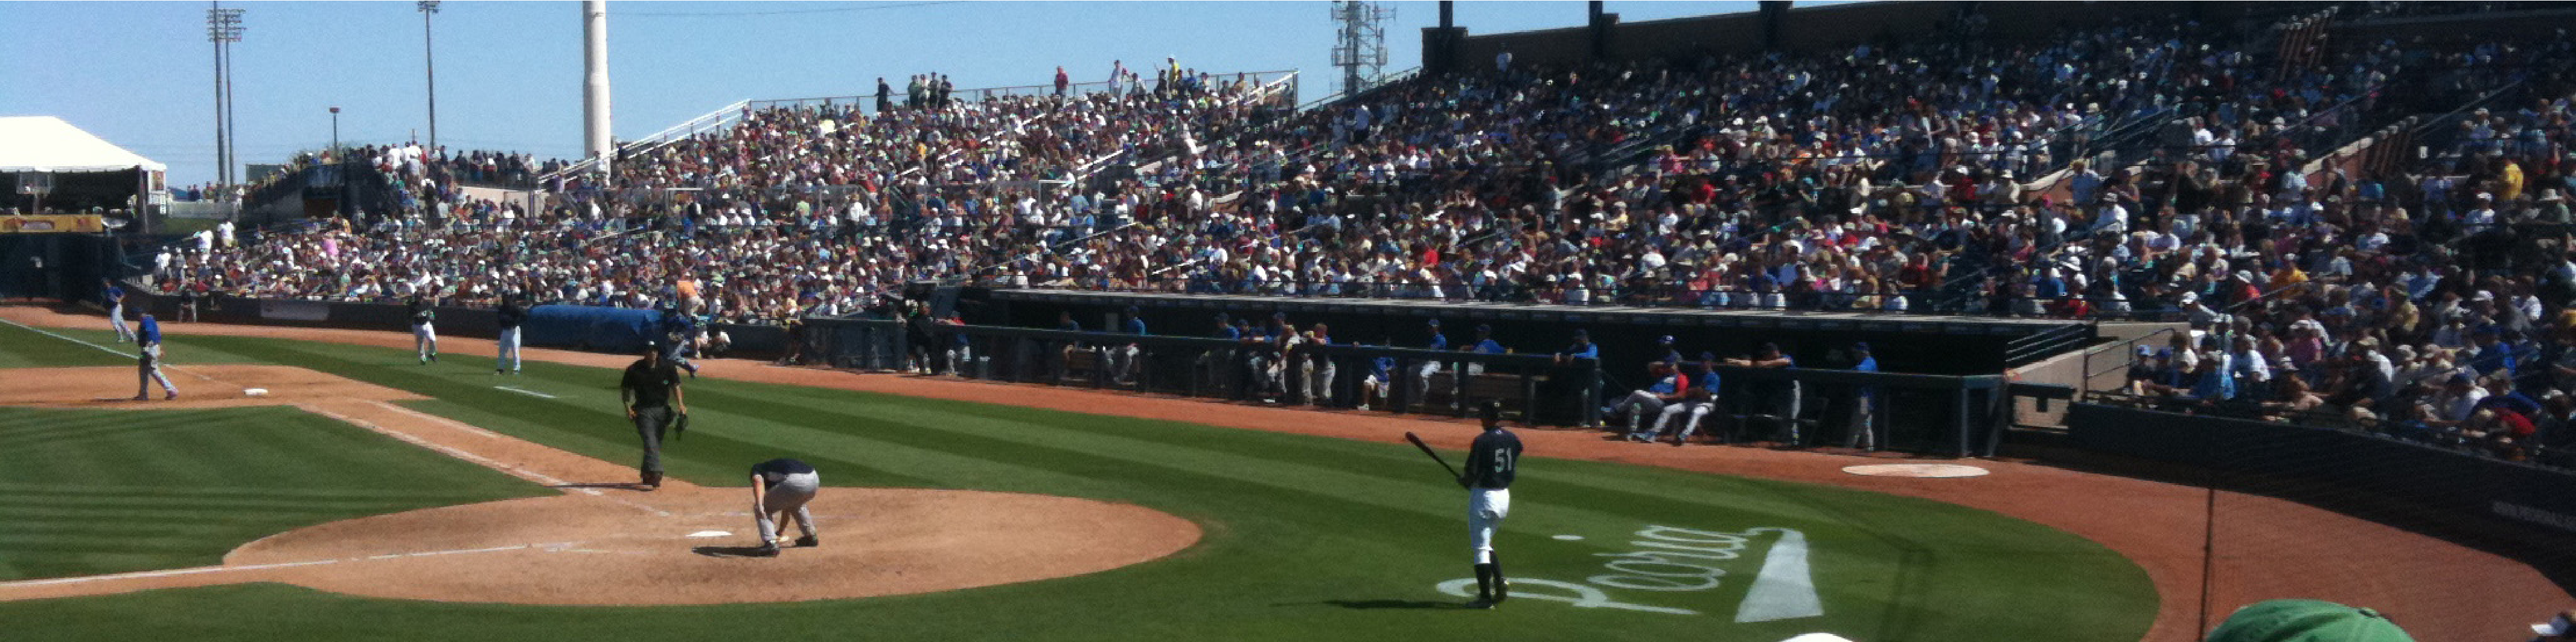
\includegraphics[width=\textwidth]{sampleteaser}
%   \caption{This is a teaser}
%   \label{fig:teaser}
% \end{teaserfigure}

\maketitle

\section{Introduction}

How do antibiotics work? Where do virus come from? What is a mutation? Can we clone people? The human kind had been studying biology for a long time but without the help of technology the revolution of the field could have been impossible. Thanks to the convergence of computation and biology, we have improved the genetic analysis discovering patterns in the genomics sequences.

The reconstruction of DNA expressions is still a significant problem in biology, and to do so firstly is needed to find all the overlapping sequences, then we can proceed to the rearrangement and reconstruction of the DNA, in order to identify from what specie do the reconstructed sequence come from.

To that end, we've come to a solution using a de Bruijn graph to represent a sequence in terms of its k-mer components and with the Eulerian path we are able find the overlapping sequences.

\section{The problem}
Every organism or living being is unique, all of them having several differences from each other, but they also have some things in common that allow us to studying them better by classifying them in certain groups, so to identify them there are certain genome sequences that define the specie. The main purpose of our project is from a collections of DNA fragments resequencing and assembling them to determine the belonging specie of the organism from the given DNA sequences.

\section{Algorithm}
\subsection{Usage}
The program is executed by command line, the first step is to insert the strings and it'll keep reading until EOF (end of file).
\subsection{Average time and memory}
The average execution time is \textbf{30} seconds.

The memory used is \textbf{15.6} mb.
\subsection{Complexity analysis}
Our solution takes a time
$O(N\times \lvert S \lvert + \lvert E \lvert + \lvert G \lvert)$.
\begin{itemize}
  \item Being $N$ the number of strings received.
  \item Being $\lvert S \lvert$ the average string length. 
  \item Being $\lvert E \lvert$ the final amount of edges in the graph.
  \item Being $\lvert G \lvert$ the final length of the resulting genome.
\end{itemize}




%\end{document}  % This is where a 'short' article might terminate

\section{RELATED WORKS}
\subsection{Longest common substring problem}
The longest common substring problem is a computer science problem in which the longest substring that two or more strings have in common needs to be found.

There are many solutions for this problem. The simpler one consists in comparing one by one all of the substrings from any of the given strings to check if it is a substring of any of the other strings and then determine which one of these is the longest.

Another solution is parsing the strings with a suffix tree and \textit{“finding the deepest internal nodes which have leaf nodes from all the strings in the subtree below it.”}

This problem can also be solved by using DP (Dynamic programming), finding which of the common suffix for all pairs of prefixes of the strings has the maximum length. The maximal of these longest common suffixes of possible prefixes must be the longest common substrings.

\subsection{Sequence alignment}
\textit{“In bioinformatics, a sequence alignment is a way of arranging the sequences of DNA, RNA, or protein to identify regions of similarity that may be a consequence of functional, structural, or evolutionary relationships between the sequences”}
This problem can be solved by the application of a variety of algorithms, so this problem has no specific solution since it can be solved by the mixture of methods and optimizations of these. An example of these algorithms and methods are DP, probabilistic or heuristic methods, etc.

\subsection{String searching for literature}
We usually need to find a specific word in an essay, chronicle or any other document with a big amount of text, that’s why engineers always try to develop every time an efficient way to satisfy this need. Here we have an example of a searching algorithm used usually for this kind of problems. 
This is the Boyer–Moore string search algorithm that was developed by Robert S. Boyer and J Strother Moore at the end of the seventies,4 this algorithm doesn’t search every character of the string, but uses a set of rules in order to minimize the time spend on the search.


\nocite{*}
\bibliographystyle{ACM-Reference-Format}
\balance
\bibliography{sigproc} 

\end{document}
